%!TEX root = ../thesis.tex
%*******************************************************************************
%****************************** Third Chapter **********************************
%*******************************************************************************
\chapter{Faser Experiment}

% **************************** Define Graphics Path **************************
\ifpdf
    \graphicspath{{ChapterFaser/Figs/Raster/}{Chapter3/Figs/PDF/}{Chapter3/Figs/}}
\else
    \graphicspath{{ChapterFaser/Figs/Vector/}{Chapter3/Figs/}}
\fi



\section{Detector location}

\nomenclature[z-FASER]{FASER}{ForwArd Search ExpeRiment}                                % first letter Z is for Acronyms
\nomenclature[z-TAS]{TAS}{Target Absorbers}
\nomenclature[z-TAN]{TAN}{Target Absorber Neutral}
\nomenclature[z-LOS]{LOS}{Line Of Sight}

The FASER collaboration discovered a disused tunnel, called TI12 (Fig. \ref{fig:infrastructure}), in just the right location to intercept these new particles that could be escaping from collisions in the ATLAS detector. The idea is that these light and weakly-interacting particles produced at the ATLAS IP will travel along the beam collision axis, unaffected by the magnets that bend the beams of particles around the ring of the LHC, through matter (mostly rock and concrete) without interacting and then interact within the FASER detector in TI12. \cite{faser_collaboration_faser:_2019} The schedule is tight. The LHC is warmed up for maintenance until end of 2020, so FASER needs to be built before RUN 3. A third long shutdown is planned for 2024 where the collaboration could do some maintenance of FASER or install FASER 2, a bigger version of FASER.

Manufacturing issues on the magnets because of the Corona virus in China have already impacted the schedule. The magnetic blocks needed for the FASER magnets will have a 2 month delay in the delivery. That puts the delivery of the 1st short magnet at the end of April and the 2nd end of May. The long magnet won't be available before end of June. This is an issue because the two short magnets form the support of the tracking detector so it is impossible to install any of the detector until they arrive. This allows more time for the commissioning of the full detector on the surface (in building ENH1). However this means the installation will be done after the cool-down period mid-July and must be completed before end of October when the LHC is handed over to LHC operations and access will be very limited. Between these dates, the tunnel will be inacessible for 2-3 weeks while some electrical tests are performed.

On Fig. \ref{fig:infrastructure} we can see that charged particles are deflected by the LHC magnets and neutral hadrons are absorbed by either the TAS or TAN. These are target absorbers designed to protect the magnets. This means that only LLPs will travel from the IP to FASER through 10 meters of concrete and 90 meters of rock. In the SM only muons and neutrinos can reach FASER. However the collaboration expects LLPs to easily pass through all of the material without interacting and decay in FASER. We also see in the bottom right corner of Fig. \ref{fig:infrastructure} that FASER will be located roughly 5 meters from the LHC tunnel.

\begin{figure}[htbp!] 
\centering    
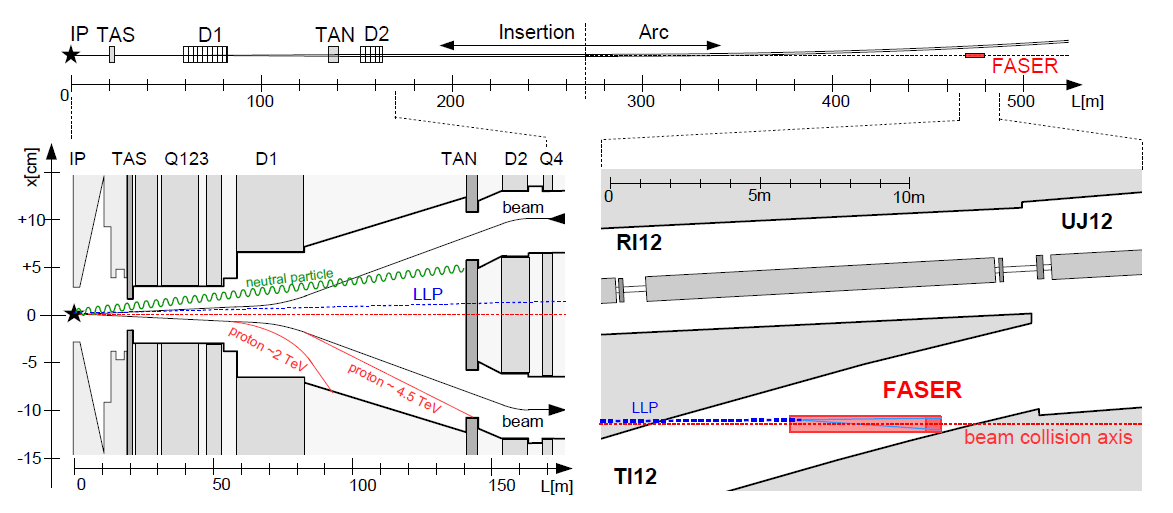
\includegraphics[width=1.0\textwidth]{FASERinfrastructureTI12.png}
\caption[TI12 infrastructure]{TI12's infrastructure}
\label{fig:infrastructure}
\end{figure}

\subsubsection{FLUKA Simulations}

Due to the bending induced by the LHC's magnets, the muon flux on LOS will be reduced. Measurement using FLUKA simulations conluded that the $\mu_{-}$ flux will be bent to the left and $\mu_{+}$ to the right of FASER, see Fig. \ref{fig:FLUKA}. These measurements were confirmed using emulsion detectors in 2018.

WHAT HAPPENS IF I WRITE THIS ?

\begin{figure}[htbp!] 
\centering    
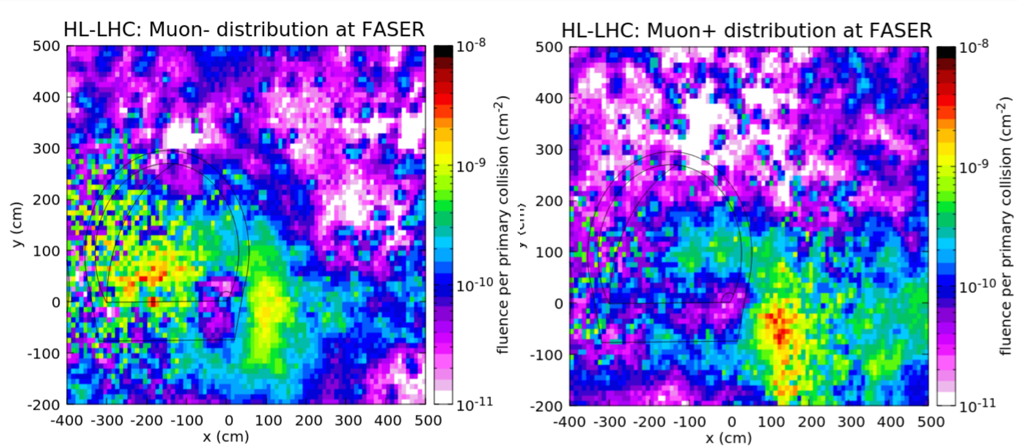
\includegraphics[width=0.8\textwidth]{FLUKA.png}
\caption[FLUKA]{FLUKA simulation}
\label{fig:FLUKA}
\end{figure}

\subsection{Civil Engineering work}

Some civil engineering works are needed. In Figs. \ref{fig:TunnelBefore} and \ref{fig:TunnelAfter} we see old ventilation conduits that have been removed. Furthermore, TI12 having a slight upwards slope, a trench need to be cut out to align FASER with the beam collision axis, see Fig. \ref{fig:CEwork} and \ref{fig:CEwork1}. The digging depth will be around 50 centimeters.

\begin{figure}[htbp!] 
\centering
\begin{minipage}{.5\textwidth}
  \centering
  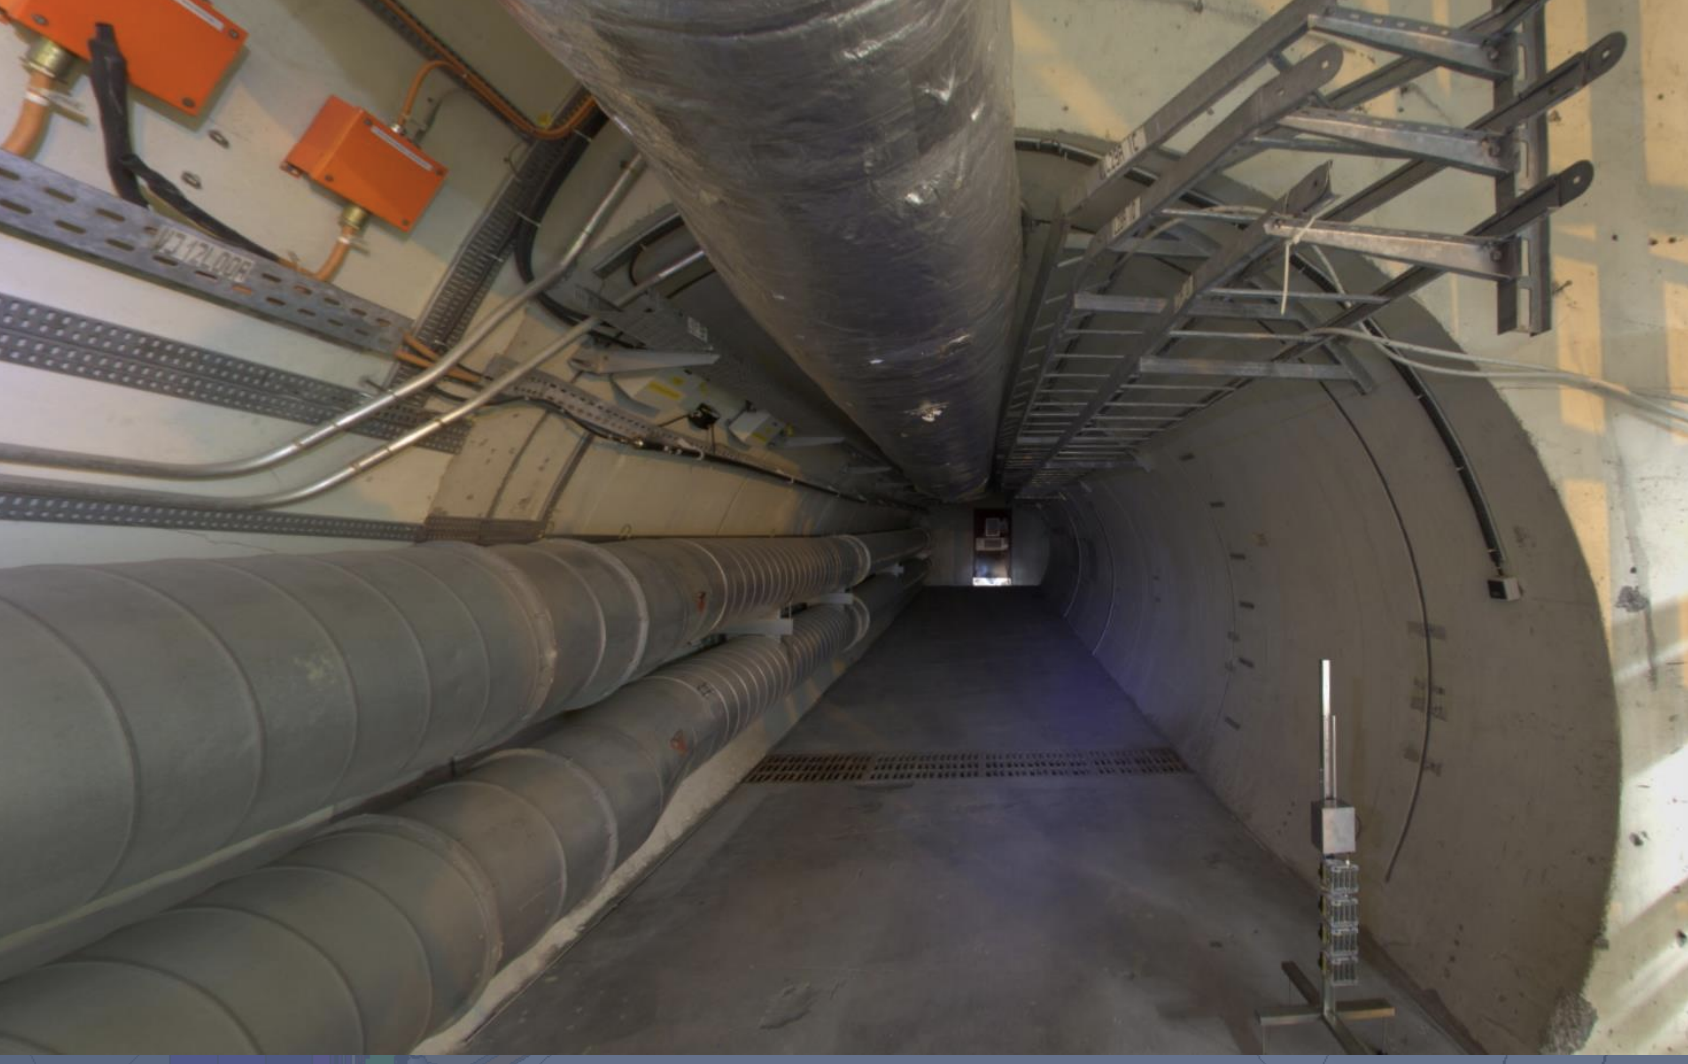
\includegraphics[width=.9\linewidth]{TunnelBefore}
  \caption[Tunnel Before]{Before}
  \label{fig:TunnelBefore}
\end{minipage}%
\begin{minipage}{.5\textwidth}
  \centering
  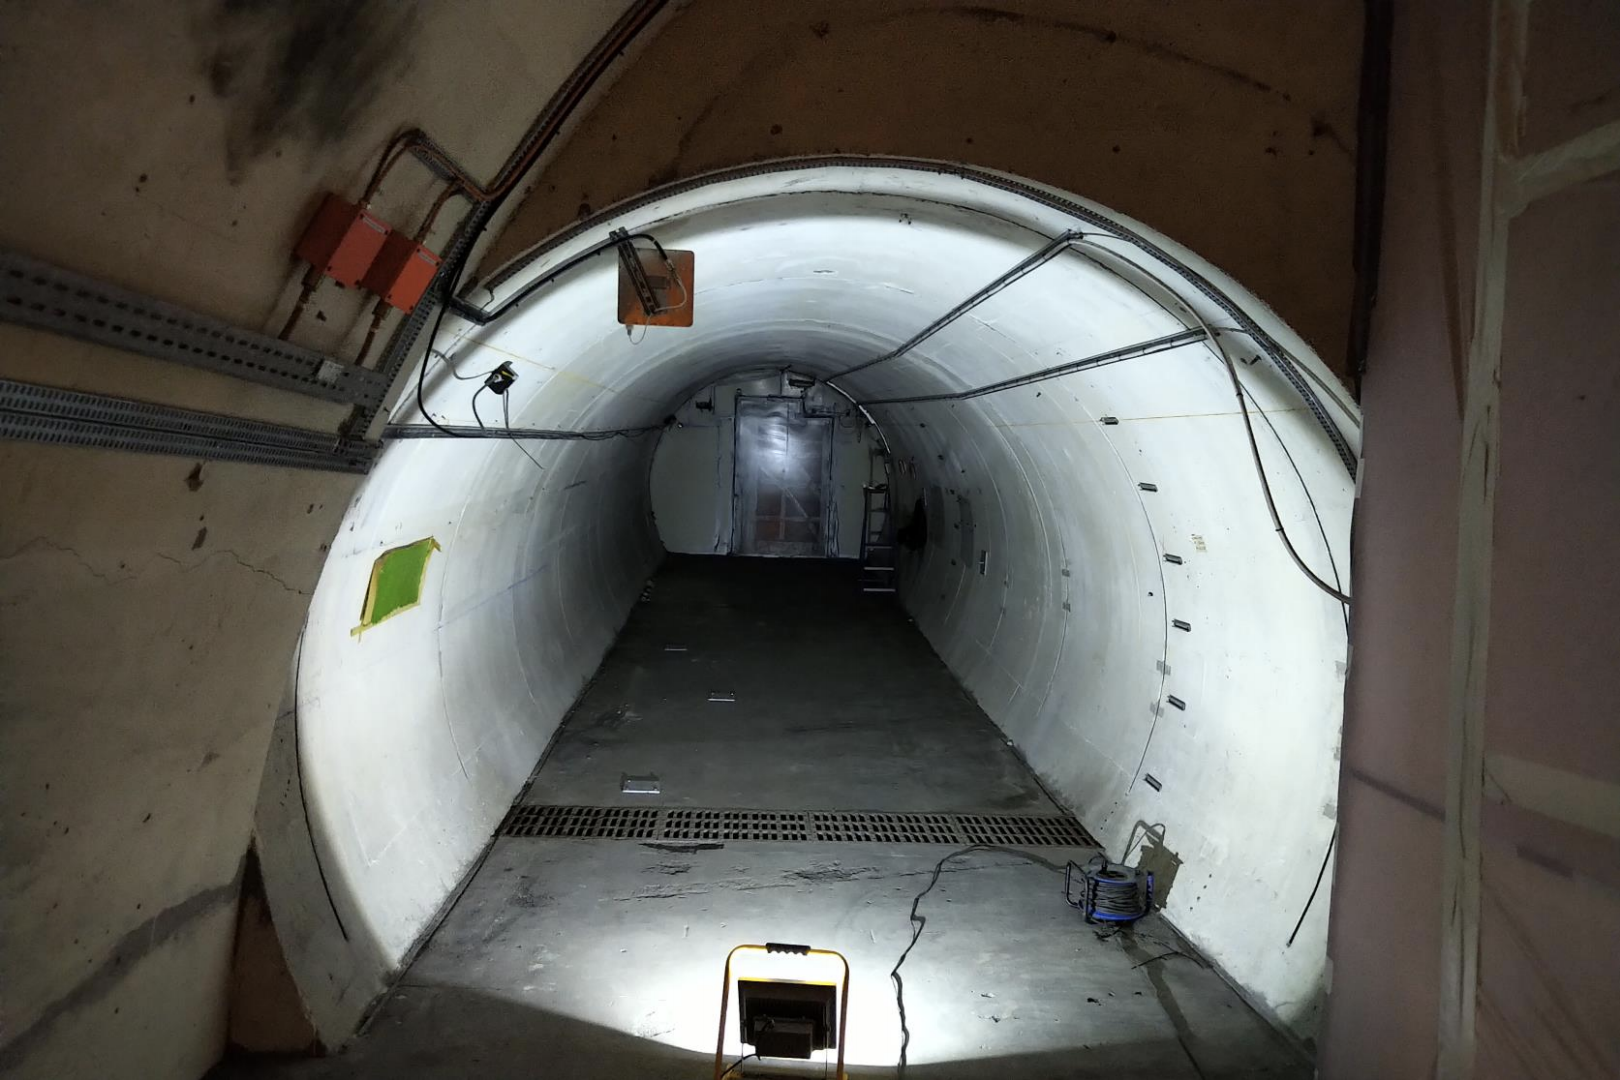
\includegraphics[width=.85\linewidth]{TunnelAfter}
  \caption[Tunnel After]{After}
  \label{fig:TunnelAfter}
\end{minipage}
\end{figure}

\begin{figure}[htbp!] 
\centering    
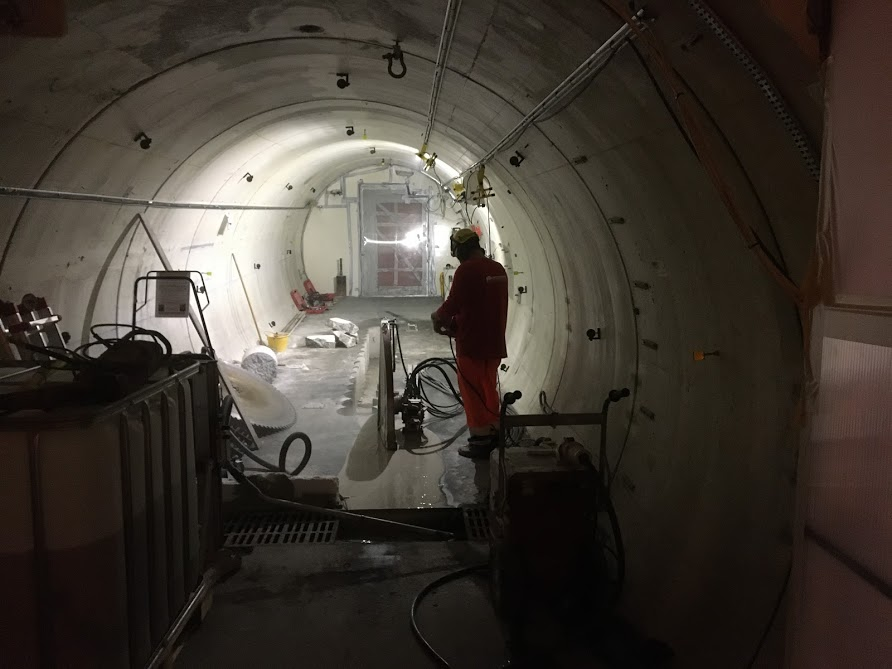
\includegraphics[width=1.0\textwidth]{ChapterFaser/Figs/Raster/CEworks.JPG}
\caption[CE work]{Civil engineering work}
\label{fig:CEwork}
\end{figure}

\begin{figure}[htbp!] 
\centering    
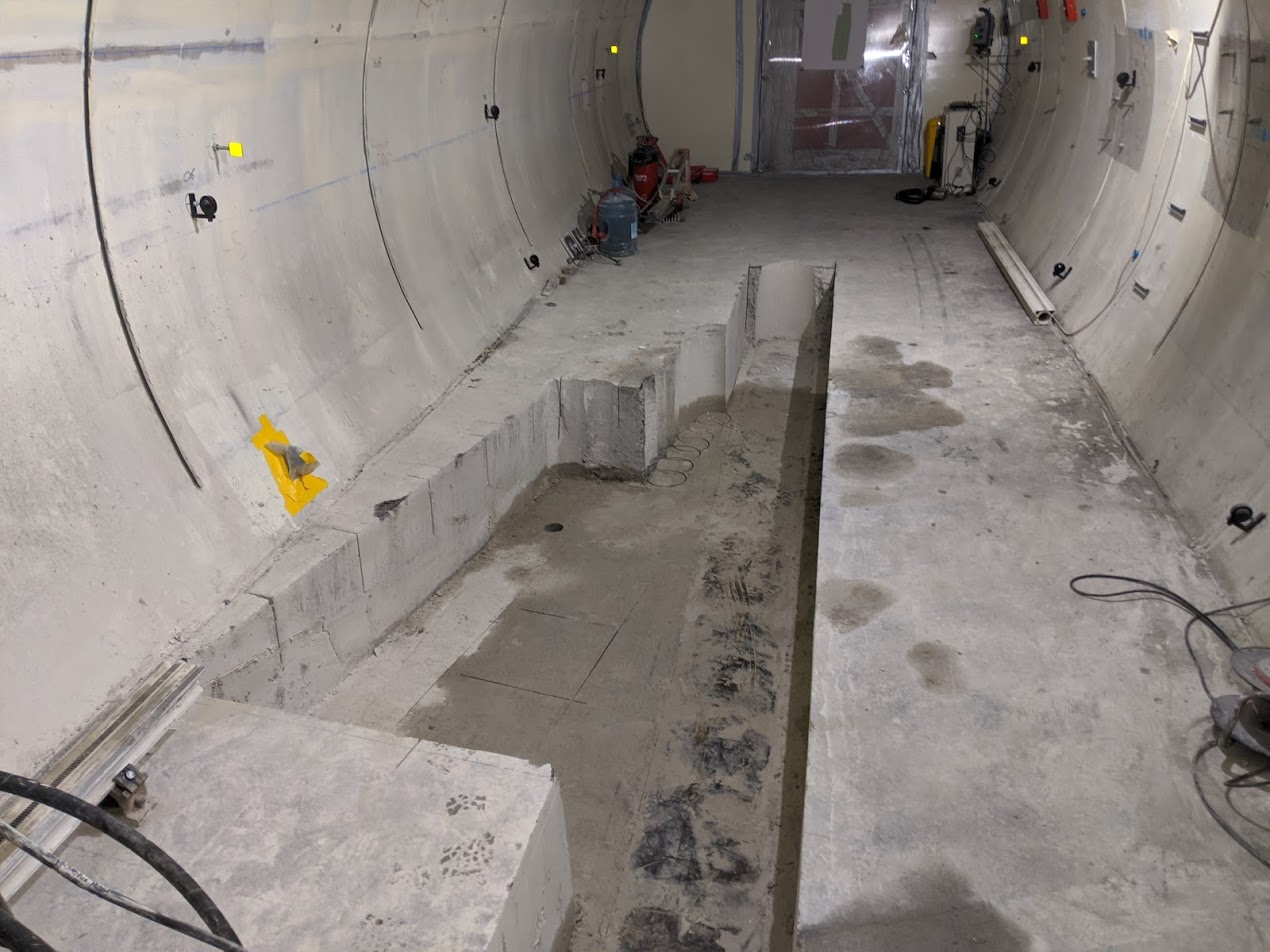
\includegraphics[width=1.0\textwidth]{ChapterFaser/Figs/Raster/CEworks1.JPG}
\caption[CE work 1]{Civil engineering work}
\label{fig:CEwork1}
\end{figure}



\section{Magnets}
and here I write more \dots
\section{Instruments - etc}
